\documentclass[]{article}
\usepackage{lmodern}
\usepackage{amssymb,amsmath}
\usepackage{ifxetex,ifluatex}
\usepackage{fixltx2e} % provides \textsubscript
\ifnum 0\ifxetex 1\fi\ifluatex 1\fi=0 % if pdftex
  \usepackage[T1]{fontenc}
  \usepackage[utf8]{inputenc}
\else % if luatex or xelatex
  \ifxetex
    \usepackage{mathspec}
  \else
    \usepackage{fontspec}
  \fi
  \defaultfontfeatures{Ligatures=TeX,Scale=MatchLowercase}
\fi
% use upquote if available, for straight quotes in verbatim environments
\IfFileExists{upquote.sty}{\usepackage{upquote}}{}
% use microtype if available
\IfFileExists{microtype.sty}{%
\usepackage{microtype}
\UseMicrotypeSet[protrusion]{basicmath} % disable protrusion for tt fonts
}{}
\usepackage[margin=1in]{geometry}
\usepackage{hyperref}
\hypersetup{unicode=true,
            pdfborder={0 0 0},
            breaklinks=true}
\urlstyle{same}  % don't use monospace font for urls
\usepackage{color}
\usepackage{fancyvrb}
\newcommand{\VerbBar}{|}
\newcommand{\VERB}{\Verb[commandchars=\\\{\}]}
\DefineVerbatimEnvironment{Highlighting}{Verbatim}{commandchars=\\\{\}}
% Add ',fontsize=\small' for more characters per line
\usepackage{framed}
\definecolor{shadecolor}{RGB}{248,248,248}
\newenvironment{Shaded}{\begin{snugshade}}{\end{snugshade}}
\newcommand{\KeywordTok}[1]{\textcolor[rgb]{0.13,0.29,0.53}{\textbf{#1}}}
\newcommand{\DataTypeTok}[1]{\textcolor[rgb]{0.13,0.29,0.53}{#1}}
\newcommand{\DecValTok}[1]{\textcolor[rgb]{0.00,0.00,0.81}{#1}}
\newcommand{\BaseNTok}[1]{\textcolor[rgb]{0.00,0.00,0.81}{#1}}
\newcommand{\FloatTok}[1]{\textcolor[rgb]{0.00,0.00,0.81}{#1}}
\newcommand{\ConstantTok}[1]{\textcolor[rgb]{0.00,0.00,0.00}{#1}}
\newcommand{\CharTok}[1]{\textcolor[rgb]{0.31,0.60,0.02}{#1}}
\newcommand{\SpecialCharTok}[1]{\textcolor[rgb]{0.00,0.00,0.00}{#1}}
\newcommand{\StringTok}[1]{\textcolor[rgb]{0.31,0.60,0.02}{#1}}
\newcommand{\VerbatimStringTok}[1]{\textcolor[rgb]{0.31,0.60,0.02}{#1}}
\newcommand{\SpecialStringTok}[1]{\textcolor[rgb]{0.31,0.60,0.02}{#1}}
\newcommand{\ImportTok}[1]{#1}
\newcommand{\CommentTok}[1]{\textcolor[rgb]{0.56,0.35,0.01}{\textit{#1}}}
\newcommand{\DocumentationTok}[1]{\textcolor[rgb]{0.56,0.35,0.01}{\textbf{\textit{#1}}}}
\newcommand{\AnnotationTok}[1]{\textcolor[rgb]{0.56,0.35,0.01}{\textbf{\textit{#1}}}}
\newcommand{\CommentVarTok}[1]{\textcolor[rgb]{0.56,0.35,0.01}{\textbf{\textit{#1}}}}
\newcommand{\OtherTok}[1]{\textcolor[rgb]{0.56,0.35,0.01}{#1}}
\newcommand{\FunctionTok}[1]{\textcolor[rgb]{0.00,0.00,0.00}{#1}}
\newcommand{\VariableTok}[1]{\textcolor[rgb]{0.00,0.00,0.00}{#1}}
\newcommand{\ControlFlowTok}[1]{\textcolor[rgb]{0.13,0.29,0.53}{\textbf{#1}}}
\newcommand{\OperatorTok}[1]{\textcolor[rgb]{0.81,0.36,0.00}{\textbf{#1}}}
\newcommand{\BuiltInTok}[1]{#1}
\newcommand{\ExtensionTok}[1]{#1}
\newcommand{\PreprocessorTok}[1]{\textcolor[rgb]{0.56,0.35,0.01}{\textit{#1}}}
\newcommand{\AttributeTok}[1]{\textcolor[rgb]{0.77,0.63,0.00}{#1}}
\newcommand{\RegionMarkerTok}[1]{#1}
\newcommand{\InformationTok}[1]{\textcolor[rgb]{0.56,0.35,0.01}{\textbf{\textit{#1}}}}
\newcommand{\WarningTok}[1]{\textcolor[rgb]{0.56,0.35,0.01}{\textbf{\textit{#1}}}}
\newcommand{\AlertTok}[1]{\textcolor[rgb]{0.94,0.16,0.16}{#1}}
\newcommand{\ErrorTok}[1]{\textcolor[rgb]{0.64,0.00,0.00}{\textbf{#1}}}
\newcommand{\NormalTok}[1]{#1}
\usepackage{longtable,booktabs}
\usepackage{graphicx,grffile}
\makeatletter
\def\maxwidth{\ifdim\Gin@nat@width>\linewidth\linewidth\else\Gin@nat@width\fi}
\def\maxheight{\ifdim\Gin@nat@height>\textheight\textheight\else\Gin@nat@height\fi}
\makeatother
% Scale images if necessary, so that they will not overflow the page
% margins by default, and it is still possible to overwrite the defaults
% using explicit options in \includegraphics[width, height, ...]{}
\setkeys{Gin}{width=\maxwidth,height=\maxheight,keepaspectratio}
\IfFileExists{parskip.sty}{%
\usepackage{parskip}
}{% else
\setlength{\parindent}{0pt}
\setlength{\parskip}{6pt plus 2pt minus 1pt}
}
\setlength{\emergencystretch}{3em}  % prevent overfull lines
\providecommand{\tightlist}{%
  \setlength{\itemsep}{0pt}\setlength{\parskip}{0pt}}
\setcounter{secnumdepth}{0}
% Redefines (sub)paragraphs to behave more like sections
\ifx\paragraph\undefined\else
\let\oldparagraph\paragraph
\renewcommand{\paragraph}[1]{\oldparagraph{#1}\mbox{}}
\fi
\ifx\subparagraph\undefined\else
\let\oldsubparagraph\subparagraph
\renewcommand{\subparagraph}[1]{\oldsubparagraph{#1}\mbox{}}
\fi

%%% Use protect on footnotes to avoid problems with footnotes in titles
\let\rmarkdownfootnote\footnote%
\def\footnote{\protect\rmarkdownfootnote}

%%% Change title format to be more compact
\usepackage{titling}

% Create subtitle command for use in maketitle
\newcommand{\subtitle}[1]{
  \posttitle{
    \begin{center}\large#1\end{center}
    }
}

\setlength{\droptitle}{-2em}

  \title{}
    \pretitle{\vspace{\droptitle}}
  \posttitle{}
    \author{}
    \preauthor{}\postauthor{}
    \date{}
    \predate{}\postdate{}
  
% header for lbg_hs2017_w13_exmsol.Rmd
\usepackage{amsmath}

\newcommand{\points}[1]
{\begin{flushright}\textbf{#1}\end{flushright}}
\newcommand{\sol}
{\vspace{2ex}\textbf{Solution}:}

\begin{document}

\thispagestyle{empty}

\begin{tabular}{l}
ETH Zurich \\
D-USYS\\
Institute of Agricultural Sciences\\
\end{tabular}

\vspace{15ex}

\begin{center}
\huge
Final Exam  \\ \vspace{1ex}
Livestock Breeding and Genomics \\  \vspace{1ex}
FS 2017 \\

\normalsize
\vspace{7ex}
Peter von Rohr 
\end{center}

\vspace{7ex}

\begin{tabular}{p{5cm}lr}
  & \textsc{Date}  & \textsc{\emph{22. December 2017}} \\
  & \textsc{Begin} & \textsc{\emph{09:15 }}\\
  & \textsc{End}   & \textsc{\emph{11:15 }}\\ 
\end{tabular}

\vspace{5ex} \large

\begin{tabular}{p{2.5cm}p{3cm}p{6cm}}
  &  Name:     &  \\
  &            &  \\
  &  Legi-Nr:  & \\
\end{tabular}

\normalsize

\vspace{9ex}

\begin{center}
\begin{tabular}{|p{3cm}|c|c|}
\hline
Problem  &  Maximal Number of Points  &  Number of Points Reached \\
\hline
1        &  48         & \\
\hline
2        &  22         & \\
\hline
3        &  30         & \\
\hline
4        &  30          & \\
\hline
5        &  29          & \\
\hline
Total    &  159    & \\
\hline
\end{tabular}
\end{center}

\clearpage
\pagebreak

\subsection{Problem 1 Relationship and
Inbreeding}\label{problem-1-relationship-and-inbreeding}

We are given the following pedigree

\begin{verbatim}
##   sire  dam
## 1 <NA> <NA>
## 2 <NA> <NA>
## 3    1    2
## 4    1    3
## 5    4    2
## 6    4    5
\end{verbatim}

\begin{enumerate}
\item[a)] Use the given pedigree to construct the numerator relationship matrix $A$
\points{36}
\end{enumerate}

\clearpage
\pagebreak

\begin{enumerate}
\item[b)] Which elements of the matrix $A$ contain the inbreeding coefficient $F_5$ of animal $5$? What is the value of the inbreeding coefficient $F_5$?
\points{8}
\end{enumerate}

\clearpage
\pagebreak

\begin{enumerate}
\item[c)] Which parents would $5$ need to have, such that $F_5 = 0$ would hold?
\points{4}
\end{enumerate}

\clearpage
\pagebreak

\subsection{Problem 2 Variance Components
Estimation}\label{problem-2-variance-components-estimation}

We are given the following dataset for the traits body weight and breast
circumference for cattle.

\begin{longtable}[]{@{}rlrr@{}}
\toprule
Animal & Herd & BodyWeight & BreastCircumference\tabularnewline
\midrule
\endhead
1 & 2 & 669 & 161\tabularnewline
2 & 1 & 635 & 144\tabularnewline
3 & 1 & 631 & 151\tabularnewline
4 & 1 & 632 & 155\tabularnewline
5 & 1 & 642 & 167\tabularnewline
6 & 2 & 676 & 165\tabularnewline
7 & 1 & 645 & 163\tabularnewline
8 & 2 & 686 & 171\tabularnewline
9 & 1 & 633 & 138\tabularnewline
10 & 1 & 641 & 170\tabularnewline
\bottomrule
\end{longtable}

\begin{enumerate}
\item[a)] What is the value for the estimated resiudal variance for the trait `body weight`, when the following assumptions are met.
\points{12}
\end{enumerate}

In a first model, we assume that \texttt{body\ weight} is influenced by
the herd leading to the following model

\[y = Xb + e\]

\begin{tabular}{lll}
wobei  &  & \\
       &  $y$  &  vector of observations for `body weight` \\
       &  $b$  &  vector of herd effects \\
       &  $X$  &  incidence matrix linking observations to herd effects \\
       &  $e$  &  vector with random resiudals with $E[e] = 0$ and $var(e) = I \sigma^2$
\end{tabular}

The estimates of the herd effects were computed using the function
\texttt{lm()} in R. The statement for that is given below

\begin{Shaded}
\begin{Highlighting}[]
\NormalTok{lm_gewicht <-}\StringTok{ }\KeywordTok{lm}\NormalTok{(BodyWeight }\OperatorTok{~}\StringTok{ }\OperatorTok{-}\DecValTok{1} \OperatorTok{+}\StringTok{ }\NormalTok{Herd, }\DataTypeTok{data =}\NormalTok{ dfWtBc)}
\KeywordTok{round}\NormalTok{(}\KeywordTok{coefficients}\NormalTok{(lm_gewicht), }\DataTypeTok{digits =} \DecValTok{1}\NormalTok{)}
\end{Highlighting}
\end{Shaded}

\begin{verbatim}
## Herd1 Herd2 
##   637   677
\end{verbatim}

\subsubsection{Your task}\label{your-task}

Estimate the residual variance \(\sigma^2\) for the given model for
\texttt{body\ weight} with the method based on the residuals. The same
value for the residual variance could also be obtained from the Output
of the \texttt{summary()}-function in R.

\clearpage
\pagebreak

\begin{enumerate}
\item[b)] What is the difference between the estimated residual variance from Problem 2a) and the estimate of the residual variance based on Maximum Likelhood? 
\points{6}
\end{enumerate}

\subsubsection{Your Task}\label{your-task-1}

\begin{itemize}
\tightlist
\item
  Describe the difference between the two estimates
\item
  Compute the value of the Maximum-Likelhood-Estimate for the residual
  variance
\item
  Which of the two estimate is considered to be ``better'' than the
  other?
\end{itemize}

\clearpage
\pagebreak

\begin{enumerate}
\item[c)] When the body weight of animal $11$ in herd $1$ was recorded, the scale broke down.  The body weight of animal $11$ is estimated such that it is within the range of $\pm 2$ standard deviations around the mean body weight for herd $1$. 
\points{4}
\end{enumerate}

\subsubsection{Hints}\label{hints}

\begin{itemize}
\tightlist
\item
  Use the estimate of the standard deviation computed from Problem 2a)
\item
  If you could not solve Problem 2a), use a value of \(10\) as an
  approximation of the estimated residuals standard deviation.
\end{itemize}

\clearpage
\pagebreak

\subsection{Problem 3 Livestock
Breeding}\label{problem-3-livestock-breeding}

\begin{enumerate}
\item[a)] What is the difference between livestock population and wildlife populations with respect to the terms `selection` and `mating`? Please complete the following table.
\points{8}
\end{enumerate}

\vspace{3ex}

\begin{center}
\begin{tabular}{p{2cm}|p{5.5cm}|p{5.5cm}}
\hline
& & \\
Population & Selection & Mating \\
& & \\
\hline
& & \\
& & \\
Wildlife &  &  \\ 
& & \\
& & \\
\hline
& & \\
& & \\
Livestock &  &  \\ 
& & \\
& & \\
\hline
\end{tabular}
\end{center}

\clearpage
\pagebreak

\begin{enumerate}
\item[b)] In a selection scheme based on phenotypic observations, the distribution of the parents and the progeny is compared in the following diagram. Please put names on the labels in the following diagram.
\points{12}
\end{enumerate}

\begin{center}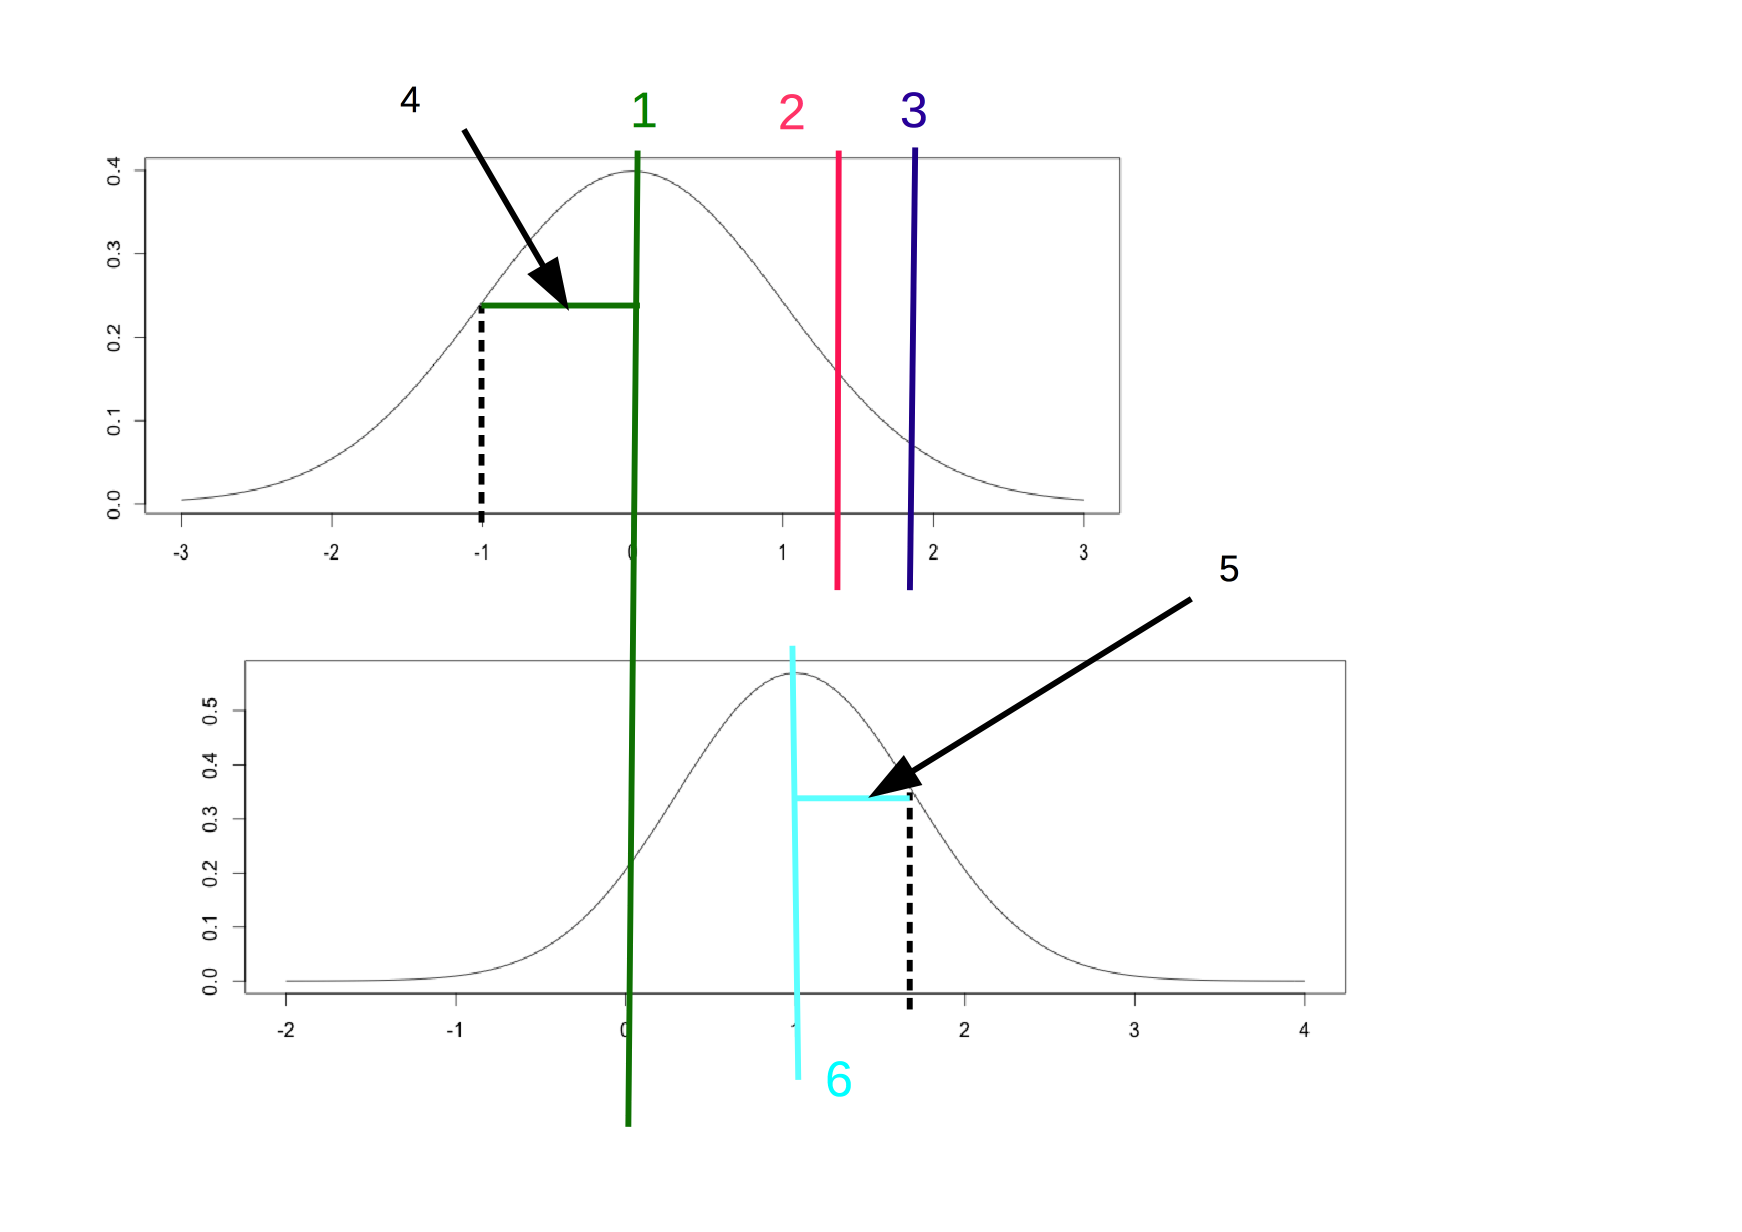
\includegraphics{png/GerichteteSelektionElternNk} \end{center}

\clearpage
\pagebreak

\begin{enumerate}
\item[c)] In pig breeding the two meat quality traits \textbf{tenderness} (ZH) and \textbf{juiciness} (SH) should be considered in the aggregate genotype $H$. The economic values for the two traits are $w_{ZH} = 5$ und $w_{SH} = 1$. Because both traits in the aggregate genotype are difficult to measure, $H$ is estimated using an index $I$ which contains the traits \textbf{sheer force} (SK) and \textbf{drip loss} (SV) beinhaltet. What is the vector $b$ of index weights which follows from selection index theory? 
\end{enumerate}

\subsubsection{Assumptions}\label{assumptions}

\begin{itemize}
\tightlist
\item
  Economic values \(w\) are given as
\end{itemize}

\[w = \left[
\begin{array}{r}
  5 \\ 
  1 \\ 
  \end{array}\right]
\]

\begin{itemize}
\tightlist
\item
  The variance covariance matrix \(P\) between the traits \texttt{SK}
  and \texttt{SV} in the index is
\end{itemize}

\[P = \left[
\begin{array}{rr}
  4 & 0 \\ 
  0 & 10 \\ 
  \end{array}\right]
\]

\begin{itemize}
\tightlist
\item
  The covariance matrix \(G\) between the traits in the index and in the
  aggregate genotype is
\end{itemize}

\[G = \left[
\begin{array}{rr}
  1.0 & -0.2 \\ 
  0.2 & 2.0 \\ 
  \end{array}\right]
\]

\subsubsection{Your Task}\label{your-task-2}

Compute the vector \(b\) of index weights.

\clearpage
\pagebreak

\subsection{Problem 4 Inbreeding}\label{problem-4-inbreeding}

\begin{enumerate}
\item[a)] The efficient computation of inbreeding in big pedigrees is baed on the Cholesky-Decomposition of the numerator relationship matrix $A$. Compute the matrix $R$ which results from the Cholesky-Decomposition for the following pedigree.
\points{25}
\end{enumerate}

\begin{verbatim}
##   sire  dam
## 1 <NA> <NA>
## 2 <NA> <NA>
## 3    2    1
## 4    2    1
## 5    3    4
\end{verbatim}

\subsubsection{Hint}\label{hint}

The Cholesky-Decomposition of the matrix \(A\) is \[A = R*R^T\]

\clearpage
\pagebreak

\begin{enumerate}
\item[b)] Compute the inbreeding coefficients of the five animals in the pedigree of Problem  4a) based on the values in matrix $R$. 
\points{5}
\end{enumerate}

\clearpage
\pagebreak

\subsection{Problem 5 Prediction of Breeding
Values}\label{problem-5-prediction-of-breeding-values}

Breeding values should be predicted based on the following data set.

\begin{longtable}[]{@{}llr@{}}
\toprule
Animal & Herd & Observation\tabularnewline
\midrule
\endhead
1 & NA & NA\tabularnewline
2 & NA & NA\tabularnewline
3 & B & 118\tabularnewline
4 & A & 120\tabularnewline
5 & A & 135\tabularnewline
6 & B & 115\tabularnewline
\bottomrule
\end{longtable}

The variances can be taken from the following table.

\begin{longtable}[]{@{}lr@{}}
\toprule
Component & Value\tabularnewline
\midrule
\endhead
phenotypic & 32\tabularnewline
additive genetic & 8\tabularnewline
\bottomrule
\end{longtable}

\begin{enumerate}
\item[a)] Predict the breeding value of the 6 animals based on their own performance where the population mean $\mu$ corresponds to the average of the phenotypic observation 
\points{9}
\end{enumerate}

\clearpage
\pagebreak

\begin{enumerate}
\item[b)] Predict the breeding values for the animals in the table above using a BLUP animal model. Set up the model and the resulting mixed model equations. Transfer the information from the data into the model by filling the numeric values into the matrices and the vectors where possible. 
\points{16}
\end{enumerate}

\clearpage
\pagebreak

\begin{enumerate}
\item[c)] What are the differences when comparing the result from Problem a) and b)?
\points{4}
\end{enumerate}


\end{document}
